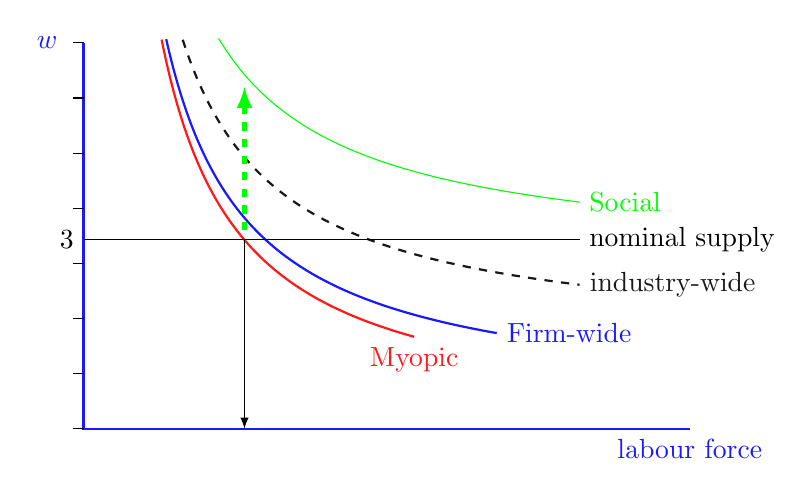
\begin{tikzpicture}[scale=.7]
%\def\bndmax{5}        %https://tex.stackexchange.com/questions/68462/filling-a-complex-region-with-tikz
%\def\bndmin{0.2}
\def \Y {7}  % height of y axis pecent
\def \W {15}  % length  of x axis
\def \Wbar {3} % jmeam wealth
\def \omega {3}
\def \A {1}  %was .5
\def \B {.5}

\draw [thick, color=blue!90] (0,\Y)node[left=.2cm]{$w$} -- (0,0)--(\W-4,0)node[below]{labour force};  
 \foreach \yi in {0,...,\Y} \draw (0,\yi)--(-.2,\yi)node[left]{};
 
\tikzset{func/.style={thick,  color=blue!90}}
% \draw[ func, domain=.2:\W-6] plot [samples=200] (\x, 2*\x^.5)node[below=.1, right]{SUPPLY};

\tikzset{func/.style={  color=green}}	
\draw[func, domain=2.45:\W-6] plot [samples=200] (\x, 10/\x+3)node[above=.1, right]{Social};

\tikzset{func/.style={thick, dashed, color=black!90}}	
\draw[func,domain=1.8:\W-6] plot [samples=200] (\x, 10/\x+1.5)node[ right]{industry-wide };

\tikzset{func/.style={thick, color=blue!90}}	
\draw[func,domain=1.5:\W-7.5] plot [samples=200] (\x, 10/\x+.4)node[below=.05, right]{Firm-wide};

\tikzset{func/.style={thick,color=red!90}}	
\draw[func,domain=8.5/6:\W-9] plot [samples=200] (\x, 10/\x)node[below]{Myopic};

\draw[](0,3.425)node[left]{$\omega$}--(9,3.425)node[right]{nominal supply };
\draw[thin,latex-](2.92,0)--(2.92,3.425); %a vertical labour supply
\draw[ultra thick,dashed, green,-latex](2.92,3.6)--(2.92,6.2);
%\draw [blue,  thick](13, 8.3)--(15,8.3)node [right, black] {\small A=\ 1,\ B=0.5};
%\draw [green, thick](13, 7.6)--(15,7.6)node [right, black] {\small A=.8, B=0.8};

%\node at (5,-1.5){Resulting in  profits, expansion, and/or entry: the city grows};
 \end{tikzpicture}